\chapter{Problem Definition and Algorithms}

In this chapter, we fomally define the problem of large query workload inefficiency in the context of temporal relational databases and then we propose a solution to lower the cost of such queries. In the next stage, we offer a practical procedure to implement the Blockchain methodology as well as the principles to add and verify trustworthiness of the records using Blockchain in a temporal relational database.

\section{Problem definition}
Keeping the historical records of transactions on a database system is useful because it stores the entire updates of a database. In our proposed system these historical records could be used to regenerate the form of a table (snapshot) or a record in a specific timestamp. Also, cryptographic techniques could be used to create a cryptographic chain in order to secure these records from tampering, therefore by investigating the authenticity of all transactions applied to an specific record throughout its lifecycle, the trustworthiness of that record could be ensured. Append-only temporal relational tables, if chosen for keeping the historical records, are beneficial because not only they are simple to implement, but also there is the luxary of having RDBMS to manage and perform queries on such tables.

\textbf{Example.} Definition of a timeline was introduced in \textbf{Definition 4}. The historical records obtained from auditing the database transaction could be seen as a timeline. A request to regenerate the form of a table (snapshot) or a record can be depicted in \ref{fig:snapshot_notion}

\begin{figure}
	\centering
	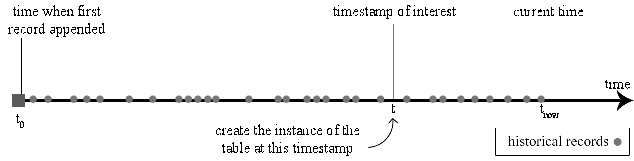
\includegraphics[width=\textwidth]{figs/snapshot_notion.pdf}
	\caption{The notion of creating snapshot on the timeline.}
	\label{fig:snapshot_notion}
\end{figure}


\textbf{Proposition. Linear time in creating snapshots}:The notion of creating a snapshot which shows the instance of the table $r$ in a certain timestamp $t$, using historical records stored in an append-only temporal relational table $r^T$ defined in \textbf{Definition 5}. Assume that the tables are updated at a constant rate over time, then the complexity of $\mathrm{snapshot}(r, t)$ is $$\mathcal{O}(|\{x: x\in r^T\mathrm{\ and\ } x.\mathrm{updates} \leq t\}|)\simeq \mathcal{O}(t)$$
Since $r^T$ could be seen as a timeline, the records which needs to be checked can be depicted in \ref{fig:checked_records}. This clearly indicates that a linear time is required to compute a snapshot at a timestamp of interest and as the size of $r^T$ grows in size, creating snapshot become computationally more expensive.

\begin{figure}[b]
	\centering
	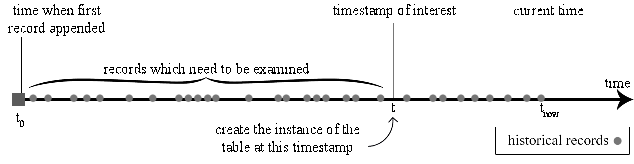
\includegraphics[width=\textwidth]{figs/tobechecked_records.pdf}
	\caption{The records which needs to be checked when creating a snapshot.}
	\label{fig:checked_records}
\end{figure}

\textbf{Example.} Given a normal relational table $r_1$ (Table \ref{table:normal_table_2}) and a temporal relational table $r_1^T$ (Table \ref{table:temporal_table_2}) which contains the historical data of $r_1$, the $r_1$ at $t=2018-04-01$ looked like Table $\ref{table:normal_table_2_t}$
\begin{center}

\begin{table}[t]
	\centering
	\caption{Normal Relational Table $r_1$}
	\label{table:normal_table_2}
	\begin{tabular}{p{4cm}p{4cm}p{4cm}}
		\hline
		id & item      & value  \\ \hline
		22 & Pencil    & 7.50 \\
		23 & Notebook & 12.0   \\ 
		24 & Console & 230.0 \\ \hline
	\end{tabular}
\end{table}

\begin{table}[t]
	\centering
	\caption{Temporal Table $r_1^T$}
	\label {table:temporal_table_2}
	\begin{tabular}{p{1cm}p{2cm}p{3cm}p{3cm}p{2cm}}
		\hline
		id & item      & value  & updated  & deleted\\ \hline
		21 & Ruler    & 3.25  & 2018-02-10  &  - \\  
		22 & Pencil    & 8.0  & 2018-03-21  &  - \\
		22 & Pencil    & 9.0  & 2018-03-30  &  -\\
		23 & Notebook & 11.0  & 2018-04-01 & - \\
		22 & Pencil & 6.0  & 2018-04-01 & - \\
		21 & Ruler    & 3.25  & -  &  2018-04-02 \\
		23 & Notebook & 12.0  & 2018-04-02 & - \\ 
		22 & Pencil & 7.50  & 2018-04-05 & - \\ 
		24 & Console & 230.0  & 2018-04-05 & - \\ \hline
	\end{tabular}
\end{table}
\end{center}
\begin{center}
\begin{table}
	\centering
	\caption{Normal Relational Table $r_1$ at t = 2018-04-01}
	\label{table:normal_table_2_t}
	\begin{tabular}{p{4cm}p{4cm}p{4cm}}
		\hline
		id & item  & value  \\ \hline
		21 & Ruler & 3.25 \\
		22 & Pencil & 6.0   \\ 
		23 & Notebook & 11.0 \\ \hline
	\end{tabular}
\end{table}
\end{center}

\subsection{Query answering using snapshots} 

Using precomputed materialized view has been proven to be effective in reducing computational time of query answering \cite{sohrabi2016materialized} \cite{du2017deepsea}. Since running queries $Q(t)$ on temporal table $r^T$ to build snapshots or generate latest version of a record at a timestamp of interest requires linear time with time complexity of approximately $\mathcal{O}(t)$, therefore in the presence of multiple and concurrent queries, such transactions are computationally expensive and inefficient. We argue that, if a snapshot is computed at the timestamp $t$ and placed on the timeline, computational time of answering to the subsequent queries on $r^T$ is reduced. The notion of having precomputed snapshots for materialization can be depicted as Figure \ref{fig:snapshot_materialization}. Note that the snapshot could exist before or after a query and in both cases the query can use the snaphsot for materialization.

\begin{figure}[t]
	\centering
	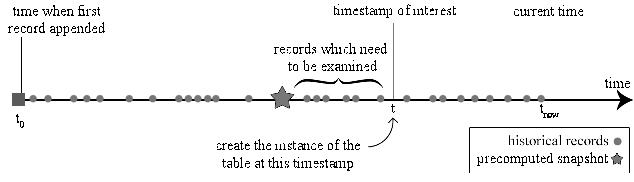
\includegraphics[width=\textwidth]{figs/snapshot_materialization.pdf}
	\caption{The records which needs to be checked when creating a snapshot with having a precomputed snapshot for materialization.}
	\label{fig:snapshot_materialization}
\end{figure}

\textbf{Proposition} suppose we have a materialized snapshot $snapshot(r,s)$. Then $snapshot(r,t)$ can be computed with complexity:
$$\mathcal{O}(|\{x: x\in r^T\mathrm{\ and\ } x.\mathrm{updates} \in [s,t]\}|) \simeq \mathcal{O}(|s-t|)$$

\textbf{Example.} Given a temporal relational table $r_1^T$ (Table \ref{table:temporal_table_3}) and a precomputed snapshot table $s_1$ at timestamp $t = 2018-03-11$(Table \ref{table:snapshot_s1}), we are interested to create a snapshot $s_2$ which is the instance of table $r_1$ at the timestamp of $t = 2018-03-15$. In order to compute snapshot $s_2$, Table \ref{table:transactions_nonmaterialized} shows the transactions which needs to be evaluated without using snapshot $s_1$ and Table \ref{table:transactions_nonmaterialized} is when $s_1$ is used for materialization. This example clearly shows that when creating snapshot $s_2$ (Table \ref{table:snapshot_s2}), less transactions need to be evaluated when $s_1$ is used for materialization.

\begin{center}
\begin{table}
	\centering
	\caption{Temporal Table $r_1^T$}
	\label {table:temporal_table_3}
	\begin{tabular}{p{1cm}p{2cm}p{3cm}p{3cm}p{2cm}}
		\hline
		id & item & value  & updated  & deleted\\ \hline
		1 & Paper & 0.25  & 2018-02-10  &  - \\  
		2 & Scissors & 8.0  & 2018-02-12  &  - \\
		3 & Folder & 1.50  & 2018-02-12  &  - \\
		1 & Paper & 0.30  & 2018-02-13  &  - \\
		4 & Pencil & 3.0  & 2018-02-16  &  - \\
		3 & Folder & 1.75  & 2018-02-21  &  - \\
		5 & Batteries & 8.0  & 2018-02-23  &  - \\
		1 & Paper & 0.35  & 2018-02-25  &  - \\
		6 & Notebook & 7.0  & 2018-03-01  &  - \\
		5 & Batteries & 9.0  & 2018-03-01  &  - \\
		4 & Pencil & 3.25  & 2018-03-04  &  - \\
		1 & Paper & 0.35  &  - &  2018-03-04 \\
		7 & Ruler & 4.0  & 2018-03-06  &  - \\
		2 & Scissors & 8.50  & 2018-03-07  &  - \\
		7 & Ruler & 4.50  & 2018-03-08  &  -\\
		5 & Batteries & 11.0  & 2018-03-10 & - \\
		3 & Folder & 1.75  & - & 2018-03-11 \\
		7 & Ruler & 4.50  & -  &  2018-03-12 \\
		6 & Notebook & 7.50  & 2018-03-15 & - \\ 
		2 & Scissors & 7.50  & 2018-03-17 & - \\ \hline
	\end{tabular}
\end{table}
\begin{table}
	\centering
	\caption{Snapshot $s_1$ at $t = 2018-03-11$}
	\label{table:snapshot_s1}
	\begin{tabular}{p{4cm}p{4cm}p{4cm}}
		\hline
		id & item  & value  \\ \hline
		2 & Scissors & 8.5   \\ 
		4 & Pencil & 3.25   \\ 
		5 & Batteries & 11.0   \\ 
		6 & Notebook & 7.0 \\ 
		7 & Ruler & 4.50   \\ \hline
	\end{tabular}
\end{table}
\end{center}

\begin{center}
\begin{table}
	\centering
	\caption{the transactions to compute snapshot $s_2$ at $t = 2018-03-15$ without using snapshot $s_1$ for materialization}
	\label{table:transactions_nonmaterialized}
	\begin{tabular}{p{1cm}p{2cm}p{2cm}p{3cm}p{2cm}p{2cm}}
		\hline
		id & item & Transaction  &timestamp & value  &query on\\ \hline
		1 & Paper & cretaed & 2018-02-10 & 0.25 & $r_1^T$ \\
		  & Paper & updated & 2018-02-13 & 0.30 & $r_1^T$ \\
		  & Paper & updated & 2018-02-25 & 0.35 & $r_1^T$ \\
		  & Paper & deleted & 2018-03-04 & - & $r_1^T$ \\ \hline
		2 & Scissors & cretaed & 2018-02-12 & 8.0 & $r_1^T$ \\
		  & Scissors & updated & 2018-03-07 & 8.50 & $r_1^T$ \\ \hline
		3 & Folder & cretaed & 2018-02-12 & 1.50 & $r_1^T$ \\
		  & Folder & updated & 2018-02-21 & 1.75 & $r_1^T$ \\
		  & Folder & deleted & 2018-03-11 & - & $r_1^T$ \\ \hline
	  	4 & Pencil & cretaed & 2018-02-16 & 3.0 & $r_1^T$ \\
		  & Pencil & updated & 2018-03-04 & 3.25 & $r_1^T$ \\ \hline
  	  	5 & Batteries & cretaed & 2018-02-23 & 8.0 & $r_1^T$ \\
		  & Batteries & updated & 2018-03-01 & 9.0 & $r_1^T$ \\
		  & Batteries & updated & 2018-03-10 & 11.0 & $r_1^T$ \\ \hline
		6 & Notebook & cretaed & 2018-03-01 & 7.0 & $r_1^T$ \\ 
		  & Notebook & updated & 2018-03-15 & 7.50 & $r_1^T$ \\ \hline
		7 & Ruler & cretaed & 2018-03-06 & 4.0 & $r_1^T$ \\
		  & Ruler & updated & 2018-03-08 & 4.50 & $r_1^T$ \\
		  & Ruler & deleted & 2018-03-12 & - & $r_1^T$ \\ \hline

	\end{tabular}
\end{table}
\end{center}

\begin{center}
\begin{table}
	\centering
	\caption{the transactions to compute snapshot $s_2$ at $t = 2018-03-15$ using snapshot $s_1$ for materialization}
	\label{table:transactions_materialized}
	\begin{tabular}{p{1cm}p{2cm}p{2cm}p{3cm}p{2cm}p{2cm}}
		\hline
		id & item & Transaction  &timestamp & value  &query on\\ \hline
		2 & Scissors & - & - & 8.50 & $s_1$ \\ \hline
	  	4 & Pencil & - & - & 3.25 & $s_1$ \\ \hline
  	  	5 & Batteries & - & - & 11.0 & $s_1$ \\ \hline
		6 & Notebook & - & - & 7.0 & $s_1$ \\ 
		  & Notebook & updated & 2018-03-15 & 7.50 & $r_1^T$ \\ \hline
		7 & Ruler & - & - & 4.50 & $s_1$ \\
		  & Ruler & deleted & 2018-03-12 & - & $r_1^T$ \\ \hline
	\end{tabular}
\end{table}
\end{center}

\begin{center}
\begin{table}
	\centering
	\caption{Snapshot $s_2$ at $t = 2018-03-15$}
	\label{table:snapshot_s2}
	\begin{tabular}{p{4cm}p{4cm}p{4cm}}
		\hline
		id & item  & value  \\ \hline
		2 & Scissors & 8.50   \\ 
		4 & Pencil & 3.25   \\ 
		5 & Batteries & 11.0   \\ 
		6 & Notebook & 7.50 \\ \hline
	\end{tabular}
\end{table}
\end{center}

\subsection{Optimal materialization of snapshots}
Let $T_q = \{q_1, q_2, \dots, q_n :q_i \in \mathcal{T}\}$ be the timestamps of $n$ queries, each querying the database at $D^T(q_i)$. To save on computational cost in answering the queries on temporal database $D^T$, we propose to compute $m$ number of snapshots $snapshot_j(r,t)$ in optimal timestamps on the timeline to answer to $T_q$ at lowest possible cost. The cost function is defined as the total query answering cost given $m$ number of precomputed snapshots. Note that $m$ is defined based on available resources in the system.

\textbf{Definition. (Cost of Query Answering)}: In the presence of a single materialized precomputed snapshot at timestamp $s \in \mathcal{T}$, the cost of answering the query $T_q$ is calculated as:
$$\mathrm{cost}(T_q | s) = \sum_{q\in T_q} |q - s|$$
Now if multiple snapshots at timestamps $S=\{s_1, s_2, \dots, s_m : s_j \in \mathcal{T}\}$ were precomputed and materialized, then 
$$\mathrm{cost}(T_q|S) = \sum_{q\in T_q} \min\{|q-s| : s\in S\}$$

\textbf{Definition. (Optimal Snapshot placement)}: For the \emph{single snapshot placement} problem, the goal is to find the timestamp $s^*$ such that 
$$cost(T_q|s)= Arg min(\sum_{q\in T_q}|q - s|)$$

The \emph{$m$-snapshot placement} problem is to compute $m$ number of timestamps $S^*=\{s_1, s_2, \dots, s_m: s_j \in \mathcal{T}\}$ to place $m$ number of snapshots for materialization, such that 
$$cost(T_q|S)= Arg min(\sum_{q\in T_q}\{|q - s|:s \in S\})$$

in the subsequent sections, we present the algorithms to address the problem of snapshot placement.

\section{Optimal single snapshot placement}
\textbf{Proposition} Let $T_q^* = {q_1,q_2, \dots , q_n}$ be $n$ number of queries performed on the temporal database. $T_q^*$ gives us a valuable insight into the query patterns on the temporal database, that could be used to find optimal position of snapshots.

\textbf{Proposition}: Given the performed queries $T_q^*$, the optimal position for a single snapshot on the timeline for materialization is $s^*(T_q^*)=median(T_q^*)$ that can be computed in $\mathcal{O}(|T_q^*|)$. Figure \ref{fig:optimal_materialization} shows the notion of placing snapshot in the median of queries for materialization.

\begin{figure}
	\centering
	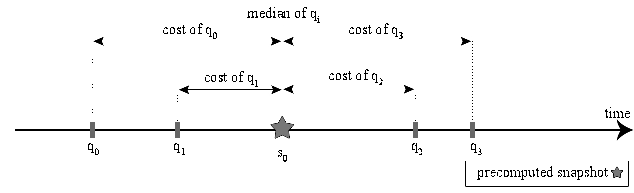
\includegraphics[width=\textwidth]{figs/optimal_materialization.pdf}
	\caption{Placing a single snapshot in the median of queries guarantees the optimal cost of query answering.}
	\label{fig:optimal_materialization}
\end{figure}

\textbf{\emph{Proof of the proposition}}:
At first, the placement of a single snapshot for two queries are discussed and then the argument is generalized for multiple queries:\\
Assume that there are two queries $T_q=\{q_1,q_2\ : q_i \in \mathcal{T}\}$ on the timeline, such that, $q_1<q_2$. for the placement of a single snapshot $s^* \in \mathcal{T}$ on the timeline, there are several cases which needs to be considered:\\
\emph{Case 1}:
$s^* \in [q_1,q_2]$, hence $q_1\leq s^*\leq q_2$.
in this case, the cost is:\\
$$cost(T_q|s^*)=\sum_{i=1}^2|q_i-s^*| = (s^*-q_1+q_2-s^*)=(q_2-q_1)$$\\
from above, it is concluded that the cost of running two queries $q_1$ and $q_2$ when snapshot is placed between them, is equal to the deviation between the two queries.\\
\emph{Case 2}:
$s^* \notin [q_1,q_2]$ and $s^* < q_1 < q_2$. for this case the cost could be calculated as follows:
$$cost_T(T_q|s^*)=\sum_{i=1}^2|q_i-s^*| = (q_1-s^*+q_2-s^*)=(q_1+q_2-2s^*) $$$$>(q_1+q_2-2q_1)=(q_2-q_1)$$\\
Therefore we conclude that if the snapshot $s^*$ is placed before queries $T_q$, the cost to perform both queries is greater than when the snapshot is placed between the two queries.\\
\emph{Case 3}:
$s^* \notin [q_1,q_2]$ and $q_1 < q_2 < s^*$.
$$cost(T_q|s^*)=\sum_{i=1}^2|q_i-s^*| = (s^*-q_1+s^*-q_2)=(2s^*-q_1-q_2) $$$$>(2q_2-q_1-q_2)=(q_2-q_1)$$\\
hence, if the snapshot $s^*$ is placed after the queries $T_q$, then the cost of performing those queries are greater than when the snapshot is placed between them.\\
From case1, case2 and case3, we can conclude that the optimal timestamp on the timeline where we can place the single snapshot $s^* \in \mathcal{T}$ to perform two queries $T_q = \{q_1,q_2:q_i\in \mathcal{T}\}$, where $q_1<q_2$ is when $s^* \in [q_1,q_2]$, meaning that $q_1 \leq s^* \leq q_2$, where the cost is equal to $q_2-q_1$.\\

Now, we generalize our conclusion from the cases that we evaluated, for the placement of a single snapshot in the presence of $n$ number of queries on the timeline: 

Suppose that there is a set of queries $T_q=\{q_1,q_2,...,q_n:q_i \in \mathcal{T}\}$ performed on the timeline. To evaluate the most optimal position to place the single snapshot $s^* \in \mathcal{T}$ for materialization, we breakdown the set of queries into the set of nested intervals $[q_1,q_n],[q_2,q_{n-1}],...,[q_i,q_{n+1-i}]$ where $n$ is the number of queries on timeline and $i=0,1,2,...,c$ where $c=\frac{n+1}{2}$ when there are odd number of queries and $c=\frac{n}{2}$ when there are even number of queries present on the timeline.\\ 
Based on the conclusion that we obtained from examining case 1, case 2 and case 3 earlier, for each nested interval, the cost of queries inside them is minimized if snapshot $s^*$ is placed in a middle of the interval. Therefore if the snapshot is placed in a position which $s^*\in \{ [q_1,q_n] \wedge [q_2,q_{n-1}] \wedge ... \wedge [q_i,q_{n+1-i}] \}$ the overall cost for all queries is minimized. In other words, if the snapshot is placed in a position that is in the middle of all nested intervals, then the total sum of absolute deviation of the snapshot from all queries is minimized. The placement of snapshot $s^*$ in the median position of $T_q$, guarantees that the snapshot is placed in the middle of all nested query intervals, where the cost of queries is calculated as follows:
$$cost(T_q|s^*)=\sum_{i=1}^n |q_i-s^*| = $$
$$[(|q_1-s^*|+|q_n-s^*|)+(|q_2-s^*|+|q_{n-1}-s^*|)+...+|q_c-s^*|+|q_{n+1-c}-s^*|)]=$$
$$[(s^*-q_1+q_n-s^*)+(s^*-q_2+q_{n-1}-s^*)+...+(s^*-q_c+q_{n+1-c}-s^*)]=$$
$$[(q_n-q_1)+(q_{n-1}-q_2)+...+(q_{n+1-c}-q_c)]$$\\
where parenthesis indicate the deviation from endpoints for one of nested intervals. In the case when there are odd number of queries performed on the timeline, the innermost interval is $[q_{\frac{n+1}{2}},q_{\frac{n+1}{2}}]$ and the position of $q_{\frac{n+1}{2}}$ is the optimal position to place snapshot $s^*$. also when there are even number of queries the innermost interval is $[q_{\frac{n}{2}},q_{\frac{n}{2}+1}]$, therefore if we choose snapshot $s^*$'s position to be at $q_{\frac{n}{2}}\leq s^*\leq q_{\frac{n}{2}+1}$,it guarantees that the snapshot exists inside each of nested intervals, and hence the sum of absolute deviation is minimized. \\

\section{Optimal multiple snapshot placement}
In the presence of thousands of queries on a temporal database with millions of records, having a single snapshot reduces the cost of query answering but it is still not enough. Therefore, to reduce the overall cost of query answring, optimal timestamps should be computed on the timeline of the temporal database to place snapshots for materialization. In the following section, different approaches to compute the optimal positions on the timeline are discussed.

\textbf{\emph{Proposition (Segmentation of queries)}}: Given an ordered set of snapshot timestamps $S=\{s_1,s_2,...,s_m:s_i \in \mathcal{T}\}$, such that $s_i \leq s_{i+1}$, and $n$ number of queries $Q = \{q_1,q_2,...,q_n: q_i \in \mathcal{T}\}$, snapshots create $m$ number of non-overlapping segments on the queries $Q[1,i_1],Q[i_1+1,i_2],...,Q[i_{m-1},i_m]$ such that queries in the segment $Q[i_j,i_{j+1}]$ use $s_j$ to answer the queries in the optimal query answering strategy. The notion of creating segmentations is depicted in Figure \ref{fig:segmentation}.

\begin{figure}
	\centering
	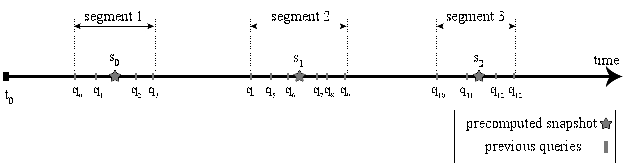
\includegraphics[width=\textwidth]{figs/segmentations.pdf}
	\caption{The notion of creating segmentations on the timeline and placing snapshot for each segmentation.}
	\label{fig:segmentation}
\end{figure}

\subsection{A recursive algorithm for optimal snapshot placements}

Let $\mathrm{opt}(Q, m)$ be the optimal $m$-snapshot placements for the query workload $Q$. Denote $Q[i,j] = \{q_i,q_{i+1},...,q_{j-1},q_j\}$.

\textbf{\emph{Proposition. (Optimality of sub-problems)}}
Let $S^* = \mathrm{opt}(Q, m)$.  Let $\mathcal{Q}$ be the partition of segments created by $S^*$.  Then, the prefix of $S^*$ is also an optimal $m-1$ snapshot placement of the prefix of $\mathcal{Q}$. Formally, $$\mathrm{prefix}(S^*) = \mathrm{opt}(\cup\mathrm{prefix}(\mathcal{Q}), m-1)$$
We can formulate a recursive definition of $\mathrm{opt}(Q, m)$ using
Proposition~\ref{thm:subopt}.  The intuition is that we try out all possible
{\em last} segment of $Q$, and pick the one with the lowest cost.

The recursive definition of $\mathrm{opt}(Q, m)$ is given as:

\begin{itemize}
	\item Base case $ \mathrm{opt}(Q, 1) = \{\mathrm{median}(Q)\}$.
	\item Induction on $m$:
	$$i^* = \mathrm{argmin}\{\mathrm{cost}(\mathrm{opt}(Q[1,i], m-1)): i\in[1,
	n]\}$$
	$$
	\mathrm{opt}(Q, m) = \mathrm{opt}(Q[1, i^*]) \cup \{\mathrm{median}(Q[i^*+1, n])
	$$
\end{itemize}
The recursive formulation of $\mathrm{opt}(Q, m)$ requires $\mathcal{O}(2^{m})$.

\textbf{Example.} Given the queries $Q=\{q_1=2,q_2=4,q_3=9,q_4=11,q_5=17,q_6=20\}$ (Figure \ref{fig:example_recursive_queries}) and maximum number of snapshots $m=3$, the goal is to find the most optimal segmentations using recursive algorithm to place snapshots for materialization. The steps to compute $m$ number of optimal segmentations is shown in Figure \ref{fig:example_recursive_steps}. In this example, the most optimal segmentation possible for 3 snapshots is when $segment_1 = \{q_0,q_1\}$, $segment_2 = \{q_2,q_3\}$, $segment_3= \{q_4,q_5\}$ where the total cost is 7 units. Figure \ref{fig:example_recursive_segmentation}.

\begin{figure}[b]
	\centering
	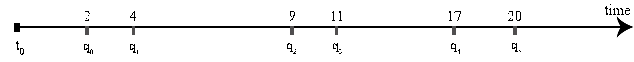
\includegraphics[width=\textwidth]{figs/example_recursive_q.pdf}
	\caption{I don't know.}
	\label{fig:example_recursive_queries}
\end{figure}

\begin{figure}
	\centering
	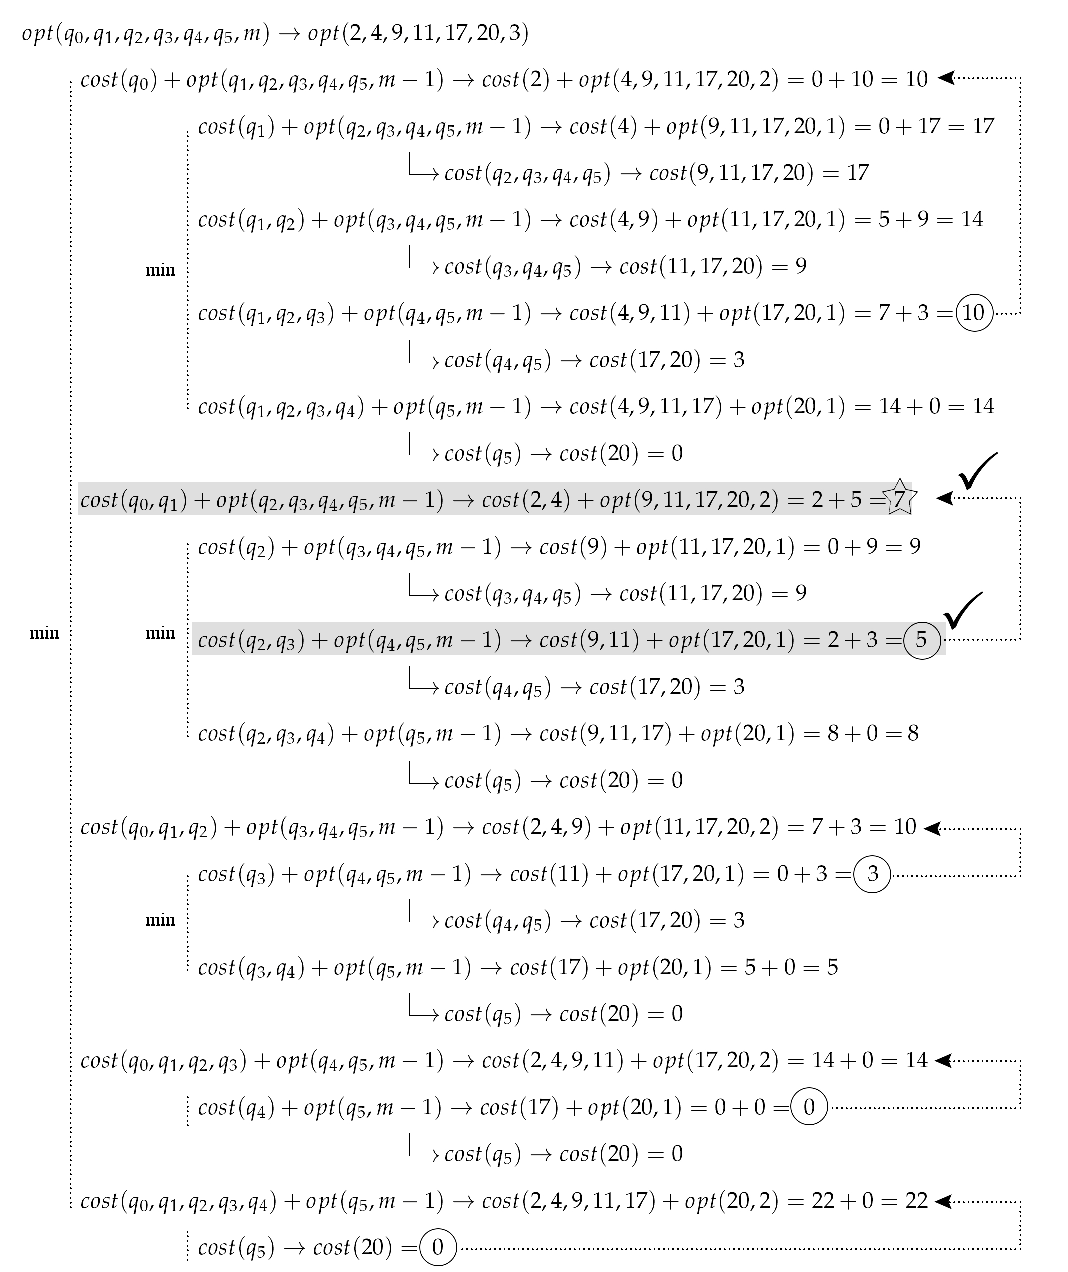
\includegraphics[width=\textwidth]{figs/recursion_example.pdf}
	\caption{Recursive approach to compute optimal segmentations for 3 snapshots.}
	\label{fig:example_recursive_steps}
\end{figure}


\begin{figure}
	\centering
	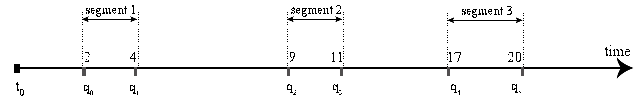
\includegraphics[width=\textwidth]{figs/example_recursive_s.pdf}
	\caption{Segmentation of queries on the timeline for Example \ref{}}
	\label{fig:example_recursive_segmentation}
\end{figure}


\subsection{Dynamic programming approach to optimal snapshot placements}

Dynamic programming improves the time complexity of finding optimal segmentations in recursive algorithm by utilizing memoization technique. In the memoization technique, if the cost of a segmentation is calculated, it is stored in a table where the recursive calls can look up the results in the table instead of recalculating them. We can build a table $\mathbf{OPT}$ as a two dimensional array
indexed by $(i, k)$ where $i\in [1, n]$ and $k\in [1, m]$.  Each entry
in the table $\mathbf{OPT}[i,k] = \mathrm{opt}(Q[1,i], k)$.
We can compute $\mathbf{OPT}[i,k]$ in a bottom up fashion \cite{}.

\begin{algorithm}[H]
\SetAlgoLined
\caption{Dynamic programming method to compute $m$ number of optimal segmentations}
\label{alg:dynamic_programming}
\DontPrintSemicolon
 \SetKwFunction{FMain}{computeOPT}
 \SetKwProg{Fn}{Function}{:}{}
 \Fn{\FMain{$Q$, $m$}}{
    $n = |Q|$\;
    \textbf{OPT}$[i,0]$ = $\infty$ \;
    \For{$k \gets 1$ \KwTo $m$}{
    	\For{$i \gets 1$ \KwTo $n$}{
    		$j^* = \underset{j\in[1,i]}{\mathrm{argmin}}(\mathrm{cost}(\mathbf{OPT}[j,k-1]) + \mathrm{cost}(Q[j+1, n]))$ \;
    		$\mathbf{OPT}[i,k] = \mathbf{OPT}[j^*, k-1] \cup \{\mathrm{median}(Q[j+1], n)\}$ 
    	}
    }
}
 
\end{algorithm}

The complexity of computing all the entries of $\mathbf{OPT}$ is $\mathcal{O}(mn^2)$.

\textbf{Example.} Given a set of queries $Q={q_0=2,q_1=4,q_2=9,q_3=11}$, we want to compute 3 segmentations from these queries, such that putting a snapshot in each segmentation, make the overall cost of answering to the queries optimal. The process of computing optimal snapshots has been showin Table \ref{table:dynamic_programming}. This method is more efficient than recursive algorithm as for example in the memoization table T[3][2], the recursive call uses the cost stored in T[2][1], T[2][2] and T[2][3] without the need to recalulate them. In this example, the most optimal overall cost is 2 which is achieved by either $\{segment1 =[q_0,q_1],segment2=[q_2],segment3=[q_3]\}$ or $\{segment1 =[q_0], segment2 = [q_1], segment3 = [q_2, q_3]\}$

\begin{table}[]
\scriptsize
\renewcommand{\arraystretch}{2}
\setlength\tabcolsep{1pt}
\caption{Memoization table T for dynamic programming approach to compute 3 optimal segmentations from 4 queries.}
\label{table:dynamic_programming}
\begin{tabular}{|l|l|l|l|l|}
\hline
0 & 0 & 0 & 0 & 0 \\ \hline

0 & $T{[}0{]}{[}0{]}+cost(q_0)$& 
$T{[}0{]}{[}1{]}+cost(q_0,q_1) $ & 
$T{[}0{]}{[}2{]}+cost(q_0,q_1,q_2)$&   
$T{[}0{]}{[}3{]}+cost(q_0,q_1,q_2,q_3) $ \\ 
 & $0+0 = 0$ & $0+2 = 2$ & $0+7=7$ & $0+14 = 14$ \\ \hline

0 & 
$T[1][0]+cost[q_0]$ & 
$min\left\{\begin{array}{ll}T[1][1]+cost[q_1] \\ T[1][2]+cost[]\end{array}\right.$&
$min\left\{\begin{array}{lll}T[1][1]+cost[q_1,q_2] \\ T[1][2]+cost[q_2] \\ T[1][3]+cost[] \end{array}\right.$&
$min\left\{\begin{array}{llll}T[1][1]+cost[q_1,q_2,q_3] \\ T[1][2]+cost[q_2,q_3] \\ T[1][3]+cost[q_3] \\ T[1][4]+cost[] \end{array}\right.$\\ 

& $0+0 = 0$ & 
$min\left\{\begin{array}{ll}  0+0 = 0 \\ 0 + 2 = 2 \end{array}\right.$ & 
$min\left\{\begin{array}{lll}  0+5 = 5 \\ 2 + 0 = 2 \\ 7+0=7  \end{array}\right.$ & 
$min\left\{\begin{array}{lll}  0+7 = 7 \\ 2 + 2 = 4 \\ 7+0=7 \\ 14+0 = 14 \end{array}\right.$ \\ \hline

0 & 
$T[2][0]+cost[q_0]$ & 
$min\left\{\begin{array}{ll}T[2][1]+cost[q_1] \\ T[2][2]+cost[]\end{array}\right.$&
$min\left\{\begin{array}{lll}T[2][1]+cost[q_1,q_2] \\ T[2][2]+cost[q_2] \\ T[2][3]+cost[] \end{array}\right.$&
$min\left\{\begin{array}{llll}T[2][1]+cost[q_1,q_2,q_3] \\ T[2][2]+cost[q_2,q_3] \\ T[2][3]+cost[q_3] \\ T[2][4]+cost[] \end{array}\right.$\\ 

& $0+0 = 0$ & 
$min\left\{\begin{array}{ll}  0+0 = 0 \\ 0 + 0 = 0 \end{array}\right.$ & 
$min\left\{\begin{array}{lll}  0+5 = 5 \\ 0 + 0 = 0 \\ 2+0=2  \end{array}\right.$ & 
$min\left\{\begin{array}{lll}  0+7 = 7 \\ 0 + 2 = 2 \\ 2+0=2 \\ 4+0 = 4 \end{array}\right.$ \\ \hline

\end{tabular}
\end{table}


\subsection{Heuristic snapshot placements}
In the heuristic technique, the optimal solution to a problem is not guaranteed however because of the low computational cost and satisfactory results, this approach is used when non-heuristic techniques are inefficient to implement. For the purpose of finding the optimal segmentation of queries for optimal query answering, we utilized K-means clustering technique.

\textbf{Proposition}: Given $T_q^* = \{q_0,q_1,...,q_n\}$ as $n$ number of queries performed on the temporal relation $r^T$, we would like to group the $q_i \in T_q^*$ into $m$ number of \textit{"clusters"}. Applying K-means clustering methodology to this problem requires to minimize the objective function defined as:
$$J = \sum_{j=1}^{m} \sum_{i=1}^{n} ||q_i^{(j)}-\mu_j||^2$$
where $\mu_j$ is the centroid of $j^{th}$ cluster and $||q_i^{(j)}-\mu_j||^2$ is the squared error function which indicates the distance between each query and their assigned centroids.
Minimizing objective function is achieved by the relocation of $\mu_j$ until no changes occur in the objective function.

\begin{algorithm}[H]
\SetAlgoLined
\caption{K-means clustering to compute $m$ number of segmentations}
\label{alg:Kmeans}
\DontPrintSemicolon
 \SetKwFunction{FMain}{K-Means}
 \SetKwProg{Fn}{Function}{:}{}
 \Fn{\FMain{$T_q^*\{q_1,...,q_n\}$, $m$}}{
    $\{\mu_1,...,\mu_m\} \gets SelectRandomSeeds(\{q_i\in T_q^*\},m)$ \;
	\For{$i \gets 1$ \KwTo $n$}{
		$J \gets argmin_{J^*}||\mu_{J^*}-q_i||^2$ \;
		$\mathcal{L}_j \gets \mathcal{L}_j \cup \{q_i\}$ 
	}
	\For{$j \gets 1$ \KwTo $m$}{
		$\mu_j \gets \frac{1}{\mathcal{L}_j} \sum_{q \in \mathcal{L}_j} q $
	}
	\Return\{$\mu_1,...,\mu_m$\}
}
\end{algorithm}

\section{Blockchain}
\subsection{Temporal database with security information}
Let $r_i^T$ be the temporal relational table with attributes $attr(r_i^T)$=$\{attr(r_i), updated,deleted\}$, denote $\alpha_u$ as the security information of the user $u$, including the user's cryptographic keys $<K_{priv}^u, K_{pub}^u>$.


\textbf{Proposition. digital signature of the transactions}. Given a set of records $rec_j =\{rec_1,rec_2,...,rec_n\} \in r_i^T$, the signature of each record could be computed as $$signature(rec_j|\alpha_u)= encrypt(hash(rec_j),K_{priv}^u)$$  

Digital signatures provide a strong mean to identify whether or not a record has been submitted by a ligitimate user. They are also used to certify if the record has not been altered as any minor change in the record results in a completely different digital signature. Also faking a digital signature is computationally infeasable, therefore digital signatures provide a strong security guarantees \cite{katz2010digital}.

\textbf{Propositin. Temporal table with chained security information}.  The temporal relational table with chained security information $r_i^{T*}$ is a table with the attributes $$attr(r_i^{T*}) = attr(r_i^T) \cup \{username,currentSignature, previousSignature)\}$$ where $username$ is the username of the user $u$ who submitted the transaction, $currentSignature = signature(rec_j)$ is the digital signature of the submitted transaction $rec_j$ by $u$ and $previousSignature = signature(rec_{j-1})$ is the signature of the previous record stored in $r_i^T$. We are interested in stroring the username of the user who submitted the transaction because it enables us to fetch the public key of the user and verify their digital signature on the submitted record.

\textbf{Proposition. Chain verification}
To verify if a chain of the records are valid, the following steps are proposed:

\begin{itemize}
	\item \textbf{step 1.} verify the $currentSignature$ of individual records.
	\item \textbf{step 2.} check if $rec_j[previousSignature] == rec_{j-1}[currentSignature]$ except for $rec_0$
\end{itemize}

A chain is said to be broken if inconsistent information being gained in any of the above steps.

\textbf{Example.} The Table \ref{temporal_blockchain_table} is an example of a temporal relational table with chained security information. With assumption that each record is a block, this table also could be depicted as Figure \ref{fig:blockchain_representation} which is the blockchian representation of Table \ref{temporal_blockchain_table}.

\begin{center}
\begin{table}
	\centering
	\footnotesize
	\caption{Temporal Table $r_1^T$ with chained security information}
	\label{temporal_blockchain_table}
	\begin{tabular}{p{0.5cm}p{0.5cm}p{1cm}p{0.5cm}p{1.7cm}p{1.7cm}p{1.5cm}p{1.5cm}p{1.5cm}}
		\hline
		r\_id & id & item      & value  & updated  & deleted & username & curSgn & prevSgn \\ \hline
		151& 21 & Ruler    & 3.25  & 2018-02-10  &  - & Bob &r3T49TR & 0\\  
		152& 21 & Ruler    & 3.25  & -  &  2018-02-20 & Alice & yu0PmER & r3T49TR\\
		153& 22 & Pencil    & 8.0  & 2018-03-21  &  - & Alice & gI90vjN & yu0PmER\\
		154& 23 & Pen    & 12.0  & 2018-03-30  &  - & Bob & 89Ec578 & gI90vjN\\
		155& 22 & Pencil & 7.50  & 2018-04-01 & - & Eve & Ipu32h6 & 89Ec578\\ \hline
	\end{tabular}
\end{table} 
\end{center}

\begin{figure}
	\centering
	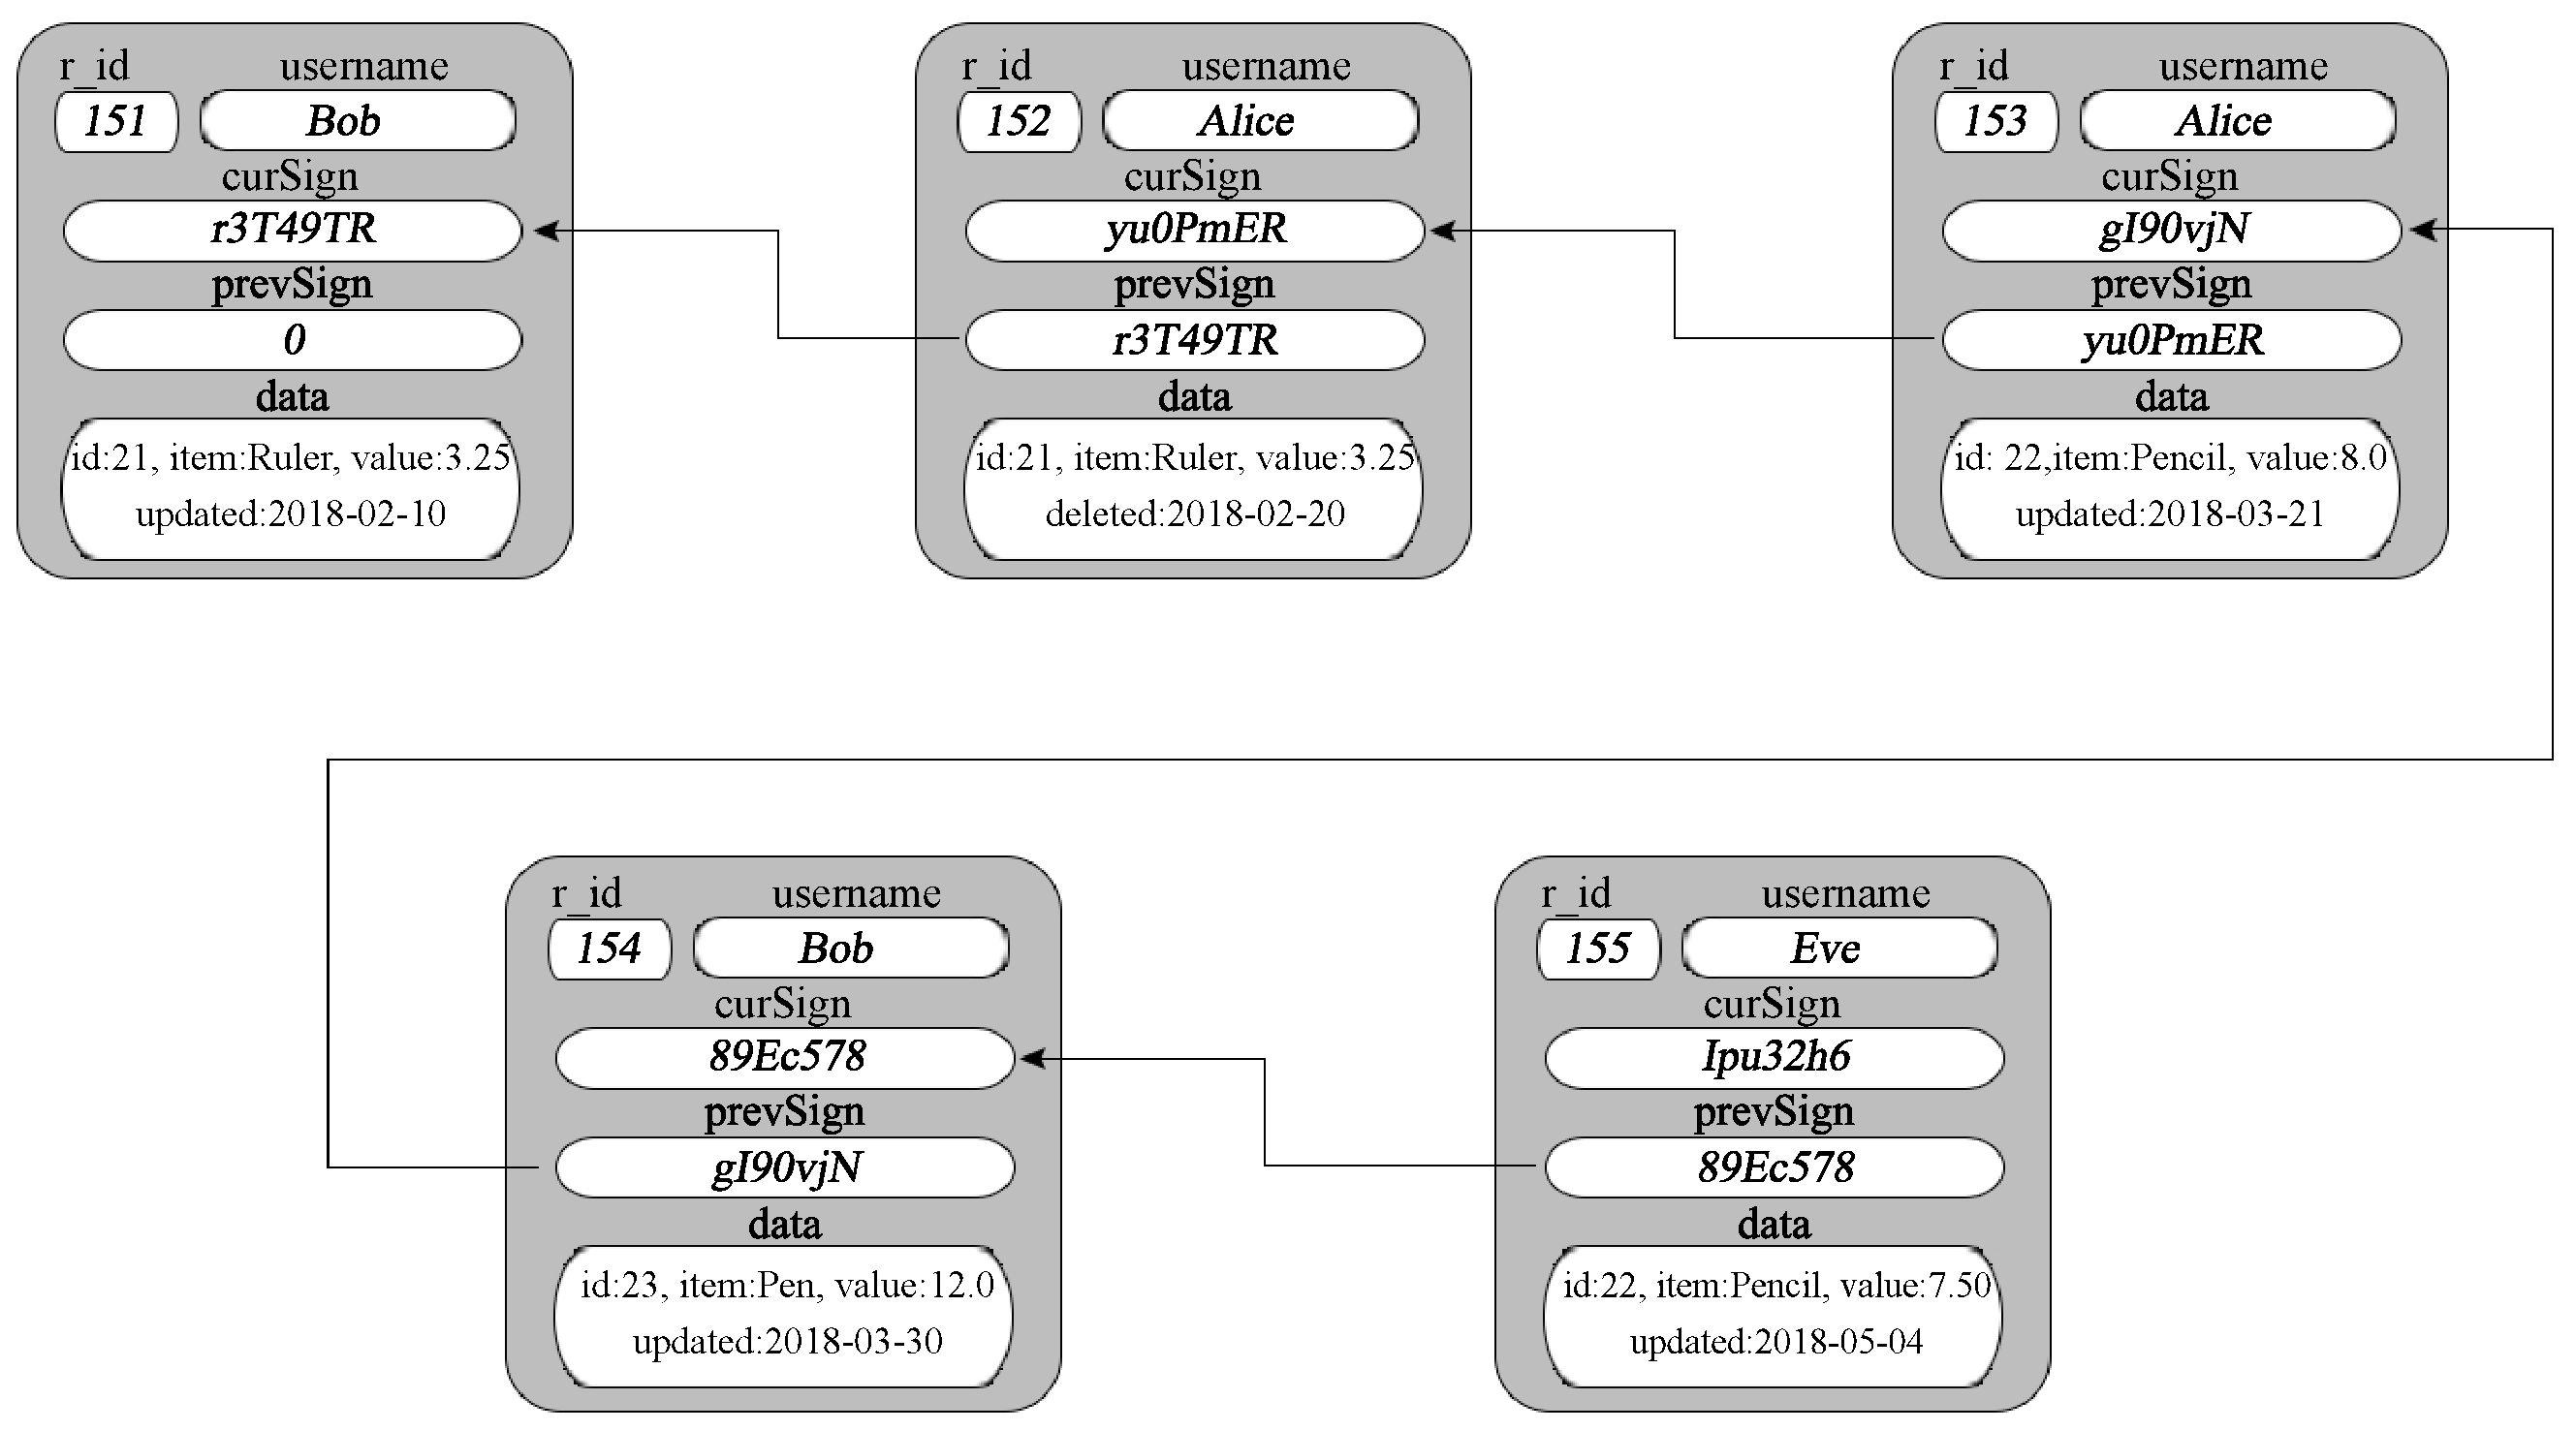
\includegraphics[width=\textwidth]{figs/temporal_blockchain.pdf}
	\caption{Blockchain representation of the table $r_1^T$.}
	\label{fig:blockchain_representation}
\end{figure}

\subsection{Trusted Snspshots}
Using blockchain to ensure the trustworthiness of data, requires a consistent chain of blocks. To make sure that a chain is consistent, all the blocks in the temporal table need to be visited and their trustworthiness need to be examined. This computation requires linear time and makes application of snapshot materialization that we discussed earlier pointless. To solve this problem, we propose the idea of trusted snapshots.

\textbf{proposition. Trusted Snapshots}. The trusted snapshot $s^*$ is a table with attributes $attr(s)\cup \{signature\}$ where $$tail(s^*[signature]) = signature(\sum_{i=0}^n (rec_i):rec_i \in s)$$

\textbf{Proposition. Trusted snaphsot materialization} We earlier talked about the materialization of snapshots for the sake of less computational time when querying the temporal database. To ensure the trustworthiness of the records while materializing trusted snapshots, we propose the following steps to be taken:
\begin{itemize}
	\item \textbf{step 1.} the signature of the materialized snapshot to be checked.
	\item \textbf{step 2.} The trustworthiness of the records which fall in between the query $q$ and snapshot $s$ to be verified using blockchain verification.
\end{itemize}
The steps which should be taken to verify the trustworthiness of the records in the case of snapshot materialization could be depicted as Figure \ref{fig:blockchain_snapshot_materialization}.

\begin{figure}
	\centering
	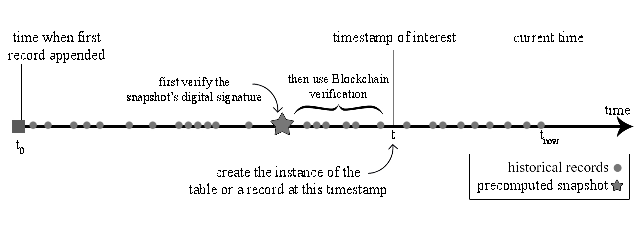
\includegraphics[width=\textwidth]{figs/trusted_snapshot_materialization.pdf}
	\caption{verify trustworthiness of the records in snapshot materialization}
	\label{fig:blockchain_snapshot_materialization}
\end{figure}

The remaining issue is that, to digitally sign the records in $s$, we need to make sure the trustworthiness of the records before hand, therefore we propose the following rules for that purpose:

\begin{itemize}
	\item The first snapshot's records trustworthiness is checked using blockchain verification.
	\item The subsequent snapshots materialize their previous snapshot, hence we take the same steps that was proposed in Proposition \ref{}
\end{itemize}

Figure \ref{fig:signing_snapshots} depicts the rules that needs to be followed when signing a precomputed snapshot.

\begin{figure}
	\centering
	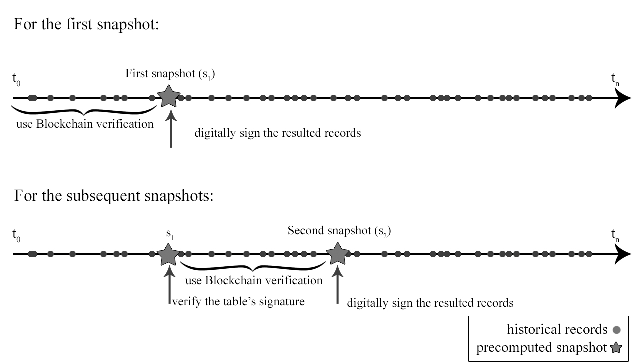
\includegraphics[width=\textwidth]{figs/signing_snapshots.pdf}
	\caption{rules that needs to be followed when signing precomputed snapshots}
	\label{fig:signing_snapshots}
\end{figure}

\section{Discussion}
In this section, the problem of linear time for query answering in append-only databases discussed. Creating snapshots and looking for the form of a table in an specific time on append-ony databases are inefficient therefore we proposed to place $m$ number of snapshots for materialization of subsequent queries. these snapshots indicate the latest version of a database until that specific time. Although it seems to be inefficient to store $m$ number of snapshots in a system, but with current cloud storages, it doesnot seem to be an overly burden task anymore. Note that $m$ is determined by checking the available resources of the host system.

In the first step, we stored the timestamp of the previous queries on the database to have the patterns of the queries on the timeline. Pattern of the queries ables us to identify the hotspots on the timeline. We argue that it is highly likeley that the the subsequent queries to be performed in these hotspots, therefore we proposed to group the queries on the hotspots and allocate one snapshot for each group for materialization. However the question which needed to be answered was to find $m$ number of optimal segmentations of queries which reduce the overall cost of answering to the queries on the temporal append-only database.

To find $m$ number of optimal segmentation, we first solved the problem of finding an optimal position to place a single snapshot. We proved that the optimal place for a single snapshot is the median of the queries, hence if $m$ number of segmentations were created, the optimal position to place snapshot within each segmentation is the median of the segmentation queries. To find the optimal segmentations we utilized three different methods : recursive algorithm, dynamic programming and K-Means clustering. Each method has their pros and cons which are shown in Table \ref{table:segmentation_comparison}. In the next section we support the comparison between methods with different experiments and we depict the observations followed by drawing a conclusion. 

\begin{center}
\begin{table}
	\centering
	\small
	\caption{Snapshot $s_2$ at $t = 2018-03-15$}
	\label{table:segmentation_comparison}
	\begin{tabular}{p{4cm}p{4cm}p{4cm}}
		\hline
		method & Pros  & Cons  \\ \hline
		Recursive algorithm & Exact optimal solution & computationally expensive for large number of queries and segmentations   \\ \hline
		Dynamic programming & Exact optimal solution & computationally expensive for large number of queries and segmentations\\ 
		  & Computationally cheaper than dynamic programming &    \\ \hline
		K-Means clustering & Fast in computation & optimal solution not guaranteed \\ \hline
	\end{tabular}
\end{table}
\end{center}